%%%%%%%%%%%%%%%%%%%%% chapter2.tex %%%%%%%%%%%%%%%%%%%%%%%%%%%%%%%%%
%
%  
%
% Use this file as a template for your own input.
%
%%%%%%%%%%%%%%%%%%%%%%%% Springer-Verlag %%%%%%%%%%%%%%%%%%%%%%%%%%
%\motto{Use the template \emph{chapter.tex} to style the various elements of your chapter content.}










\chapter{Constant Depth Circuit Lower Bounds}
\label{hastad} % Always give a unique label
% use \chaptermark{}
% to alter or adjust the chapter heading in the running head

\section{Defining constant depth circuits}
Recall that the depth of a circuit is the maximal length of a path from a leaf to the output node.

Here is an example of a circuit of depth 3:
\begin{figure}
    \centering
    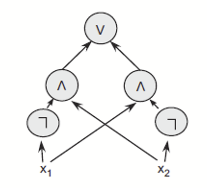
\includegraphics[width=0.25\linewidth]{images/depth 3 circuit.png}
    \label{fig:enter-label}
\end{figure}

Recall that we are interested in the asymptotic study of circuit families, not a single circuit. That is, we want to consider how circuit size grows when the number of inputs $n$ to a family of Boolean functions grows.

We can consider circuits of constant depth. This means that the depth of the circuit is \emph{independent of the number of inputs} $n$. In other words,  while $n$ the number of input gates can grow to infinity in the Boolean circuit family $\{C_n\}_{n=1}^\infty$, the depth of each circuit $C_n$ stays the same!


Note: If the depth of the circuit is constant \& the fan-in of gates is at most 2, then the number of functions we can compute w/ such constant-depth circuits is constant. For example, the number of variables (appearing as leaves, i.e., input nodes) is constant that way, so for a large enough number of inputs $n$, we will not be able to compute functions that read all the $n$ inputs.  
Thus, this model is \emph{not} complete: for a constant $d$, a depth-$d$ circuit cannot compute all Boolean functions over $n$ inputs for every $n \in \mathbb{N}$.

Corollary: To make the model of const. depth
meaningful we allow \textit{unbounded} fan-in gates:

Unbounded fan-in AND $\left(\varphi_1 \wedge \varphi_2 \wedge \ldots \wedge \varphi_\ell\right)$:
\begin{figure}
    \centering
    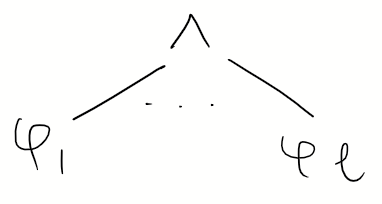
\includegraphics[width=0.2\linewidth]{images/AND.png}.
    \label{fig:enter-label}
\end{figure}

Unbounded fan-in OR $\left(\varphi\lor \cdots \lor \varphi_{\ell}\right)$:
\begin{figure}
    \centering
    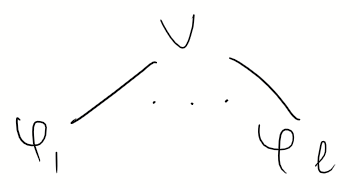
\includegraphics[width=0.25\linewidth]{images/OR.png}
.
    \label{fig:enter-label}
\end{figure}
Where $\varphi_i$'s are circuits (of constant depth) by themselves, with possibly \emph{joint} nodes. 


\begin{svgraybox}
\textbf{Important:}  When speaking about constant-depth circuits, we assume by default the fan-in of $\lor, \land$ is \emph{unbounded}. ($\neg$ has fan-in one as always.)
\end{svgraybox}

% Always give a unique label
% and use \ref{<label>} for cross-references
% and \cite{<label>} for bibliographic references
% use \sectionmark{}
% to alter or adjust the section heading in the running head
